\documentclass[11pt]{article}

% Included packages:
\usepackage{float}
\usepackage{graphicx}
\graphicspath{ {figs/} }

% Document definitions:
\setlength{\oddsidemargin}{1in}
\setlength{\evensidemargin}{1in}
\setlength{\marginparwidth}{0.0in}
\setlength{\topmargin}{0.5in}
\setlength{\headheight}{0in}
\setlength{\headsep}{0in}
\setlength{\textwidth}{4.5in}
\setlength{\textheight}{7.5in}
\setlength{\parindent}{0.25in}
\setlength{\parskip}{0.0in}
\newfont{\hvb}{cmssbx10}
\newfont{\hv}{cmss10}
\newfont{\tir}{cmr10}
\setlength{\baselineskip}{10pt}

	

%%%%%%%%%%%%%%%%%%%%%%
%%% BEGIN DOCUMENT %%%
%%%%%%%%%%%%%%%%%%%%%%
\begin{document}
\begin{center}
% Title And Authors:
{\footnotesize{\hvb
Optimizing Settling Time for Swarm UAV Formation Control In the Presence of Obstacles\\
}}

\vspace{10pt}
{\footnotesize
{\hvb Raj Shah}, {\hv M.S. Student (Mechanical)} \\
{\hvb Supreet Kurdekar}, {\hv M.S. Student (Mechanical)}\\
{\hvb Chris Gnam}, {\hv Ph.D. Student (Aerospace)} \\
{\hv
Department of Mechanical and Aerospace Engineering
University at Buffalo
Buffalo, New York, 14261
}}
\end{center}
UAVs are used in a wide range of applications such as land surveys, search and rescue operations, remote sensing, disaster monitoring to and security applications. A group of UAVs greatly enhances the performance and robustness in fulfilling difficult tasks.  Multiple agents increase the chances of completing a mission as other agents can continue the mission even if one or more agents fail.  Many of these applications require maintaining a desired formation.  Therefore it is essential that any deviations from formation keeping (such as obstacle avoidance) be kept brief.  

Our work is aimed towards optimizing settling time in formation control of UAVs swarm navigation in the presence of obstacles.  Decreased settling time in response to obstacle avoidance means less interruption to nominal operations.  This can lead to increased performance or increased quality of data collection, depending on the objective of the drone swarm. 

In \textit{Flocks, Herds, and Schools: A Distributed Behavioral Model } (Reynolds), A decentralized flock motion scheme is implented to simulate the motion of an entire flock.  This is accomplished by having each agent follow three simple rules.  \textbf{Avoidance:} avoid collisions with nearby flockmates.  \textbf{Velocity Matching:} attempt to match velocity with nearby flockmates.  \textbf{Flock Centering:} attempt to stay close to nearby flockmates.

In \textit{Stable Flocking of Mobile Agents} (Tanner), a simple methodology for stable flocking configurations was introduced, utilizing potential functions for mediating inter-agent formation keeping maneuvers.  While this method proved powerful for both acquiring and maintaining a stable flocking formation, it did not consider obstacles in its formulation.

In \textit{Virtual Leaders, Artificial Potentials and Coordinated Control of Groups} (Leonard and Fiorelli), the concept of a virtual leader was introduced.  A virtual leader is an artificial point that maintains formation shape by attracting individual agents towards itself.  This also proves advantageous as the motion of the entire swarm can be affected by controlling the virtual leader. 

Finally, in \textit{Unmanned aerial vehicle swarm control using potential functions and sliding mode control}, the use of potential functions are again used.  A repulsive potential is created around the obstacle, while potentials around each agent are used to mimic a spring like force to obtain a desired distance.  Typically, each agent has a potential applied to it and the control input for that agent uses a steepest gradient policy so as to minimize the potential function value.  Minimizing this potential function results in the agents both avoiding each other and obstacles, while also achieving the desired formation.

For the purposes of this project, we will be simulating 4 agents in 2-d space, capable of controlling their position and velocity via applied accelerations.  The agents will be following a virtual leader, which itself is following a predetermined trajectory through the environment.  The environment will have a single circular obstacle that the agents must avoid, while still following the virtual leader.

The aim is to have the agent's formation converge in as short a period of time.  The flock formation will be parameterized by a \textit{formation vector}, which is composed of all the differences between the agents and the virtual leader.  The formation is said to settle when the final \textit{formation vector} is less than 2\% different from the initial \textit{formation vector}.  The expected outcome of the project is to determine the control gains and parameters which minimize the settling time for this setup.

We will also be assuming perfect state knowledge of all the agents, and perfect knowledge of the environment.  There will be no delay or limitations on sensor speed.  However, actuation authority and velocity limitations will be applied so as to accurately capture the dynamics.

In order to accomplish this, we will be defining an objective function for the settling time, with respect to the control gains and the reaction distance from the obstacle.  The first constraint is that the vehicles must not collide with either each other or with the obstacle.  Secondly, the vehicles will have a maximum allowable acceleration (applied actuation), and will have a maximum allowable traveling velocity.

The simulation for this project will primarily be done in MATLAB.  Preliminary work has already been started implementing the papers we previously discussed so we can develop a better working knowledge of the problem.  As the project progresses, we may switch to a higher fidelity model (such as 3d space with full drone dynamics), if time allows.

The tasks of this project will be distributed among the group members.  All three members will be involved with both the formulation of the optimization problem, as well as the writing of the final report.  The project git repository, as well as the main architecture of the code, will be maintained by Chris.  Raj will focus on the implementation of simulation models, as well as continued literature review.  Supreet will be tasked primarily with designing the overall problem to be optimized, and the implementation of that into MATLAB.

\begin{figure}[H]
  \makebox[\textwidth][c]{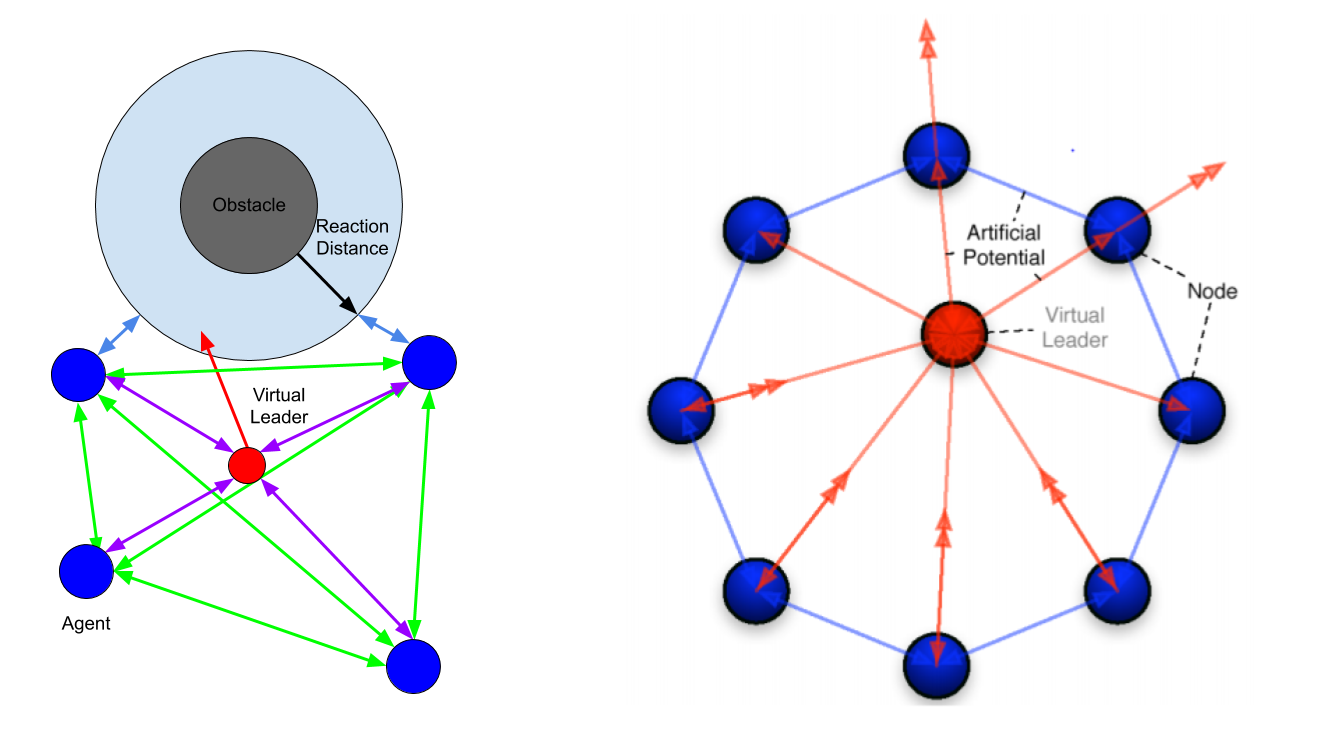
\includegraphics[width=1.2\textwidth]{MAE550_Diagram.png}}%
  \caption{Diagram of problem interactions.  \textbf{Left:} All interaction forces which define the control input.  Blue forces are agent-obstacle interactions, purple are agent-virtual leader interactions, and green are inter-agent interactions.  \textbf{Right:} Shows more clearly how the interaction forces are modeled as spring forces.  (Source: \textit{A Lightweight Formation Control Methodology for a Swarm of Non-Holonomic Vehicles})}
  \label{fig:key}
\end{figure}
\end{document}
\end{document}

